\subsection{Modality Contribution and Input Dependence}
We analyze all 669 CTCH test cases at seed 42, including incorrect predictions, using 24 IG interpolation points. Interventions remove $16\times16$ image patches or text content units while fixing the other modality. Each model retains its original predicted class as the target, with 16 random deletion orders per case.

Figure~\ref{fig:ig} shows lower targeted than random deletion AUC for images (0.2997 versus 0.3405) and text (0.2811 versus 0.3588). Whole-source replacement reduces predicted-class probability by 0.3187 for images and 0.2725 for text on average. These results indicate dependence on both inputs under the specified interventions. They neither establish region--word correspondence nor quantify cross-modal interaction. Different intervention units and references also preclude directly ranking the modalities by their deletion gaps.

XBone-Net has higher image insertion AUC than Image-only (0.4023 versus 0.2517), but also higher deletion AUC (0.2997 versus 0.1541). Because these values depend on model confidence and target class, they do not establish superior explanation quality. Lesion annotations, controlled history perturbations, and clinician review remain necessary to assess clinical plausibility.

\begin{figure*}[t]
\centering
\begin{tikzpicture}
\begin{groupplot}[
group style={group size=2 by 1,horizontal sep=13mm},
width=.46\textwidth,height=38mm,
xmin=0,xmax=1,ymin=0,ymax=.65,
xtick={0,.5,1},ytick={0,.2,.4,.6},
xlabel={Fraction removed},
axis lines=left,axis line style={black!60},
ymajorgrids,grid style={black!12},
tick label style={font=\footnotesize},
label style={font=\footnotesize},title style={font=\small\bfseries},
legend style={font=\scriptsize,draw=none,fill=none,at={(.98,.98)},anchor=north east},
]
\nextgroupplot[title={(a) Image patches},ylabel={Predicted-class probability}]
\addplot[color=red!70!black,line width=1.1pt] table[x=fraction,y=targeted]{ig_image.dat};
\addplot[color=blue!65!black,line width=1pt,dashed] table[x=fraction,y=random]{ig_image.dat};
\node[anchor=south west,font=\footnotesize,align=left] at (axis cs:.035,.025) {AUC gap: 0.0409};
\nextgroupplot[title={(b) Clinical-text units}]
\addplot[color=red!70!black,line width=1.1pt] table[x=fraction,y=targeted]{ig_text.dat};
\addlegendentry{IG-targeted deletion}
\addplot[color=blue!65!black,line width=1pt,dashed] table[x=fraction,y=random]{ig_text.dat};
\addlegendentry{Random deletion}
\node[anchor=south west,font=\footnotesize] at (axis cs:.035,.025) {AUC gap: 0.0777};
\end{groupplot}
\end{tikzpicture}

\caption{IG-guided deletion on all 669 CTCH test cases (seed 42). Curves average original predicted-class probabilities and compare IG order with 16 random orders per case. AUC gaps are random minus targeted deletion AUC. Each intervention fixes the other modality.}
\label{fig:ig}
\end{figure*}


Figure~\ref{fig:ig_case} illustrates CTCH case 3563, correctly classified as finger fracture with probability 0.5005. The author-selected example displays image relevance and signed word contributions for the same prediction. Relevance also extends beyond bone structures, illustrating the distinction between input sensitivity and validated lesion localization.

\begin{figure*}[t]
\centering
\begingroup
\centering
{\small\textbf{CTCH case 3563: Finger fracture} $\vert$ Prediction: Finger fracture (50.0\%)}\par\smallskip
\begin{minipage}[t]{0.185\linewidth}
\centering\vspace{0pt}
{\footnotesize\textbf{(a) Radiograph}}\par\smallskip
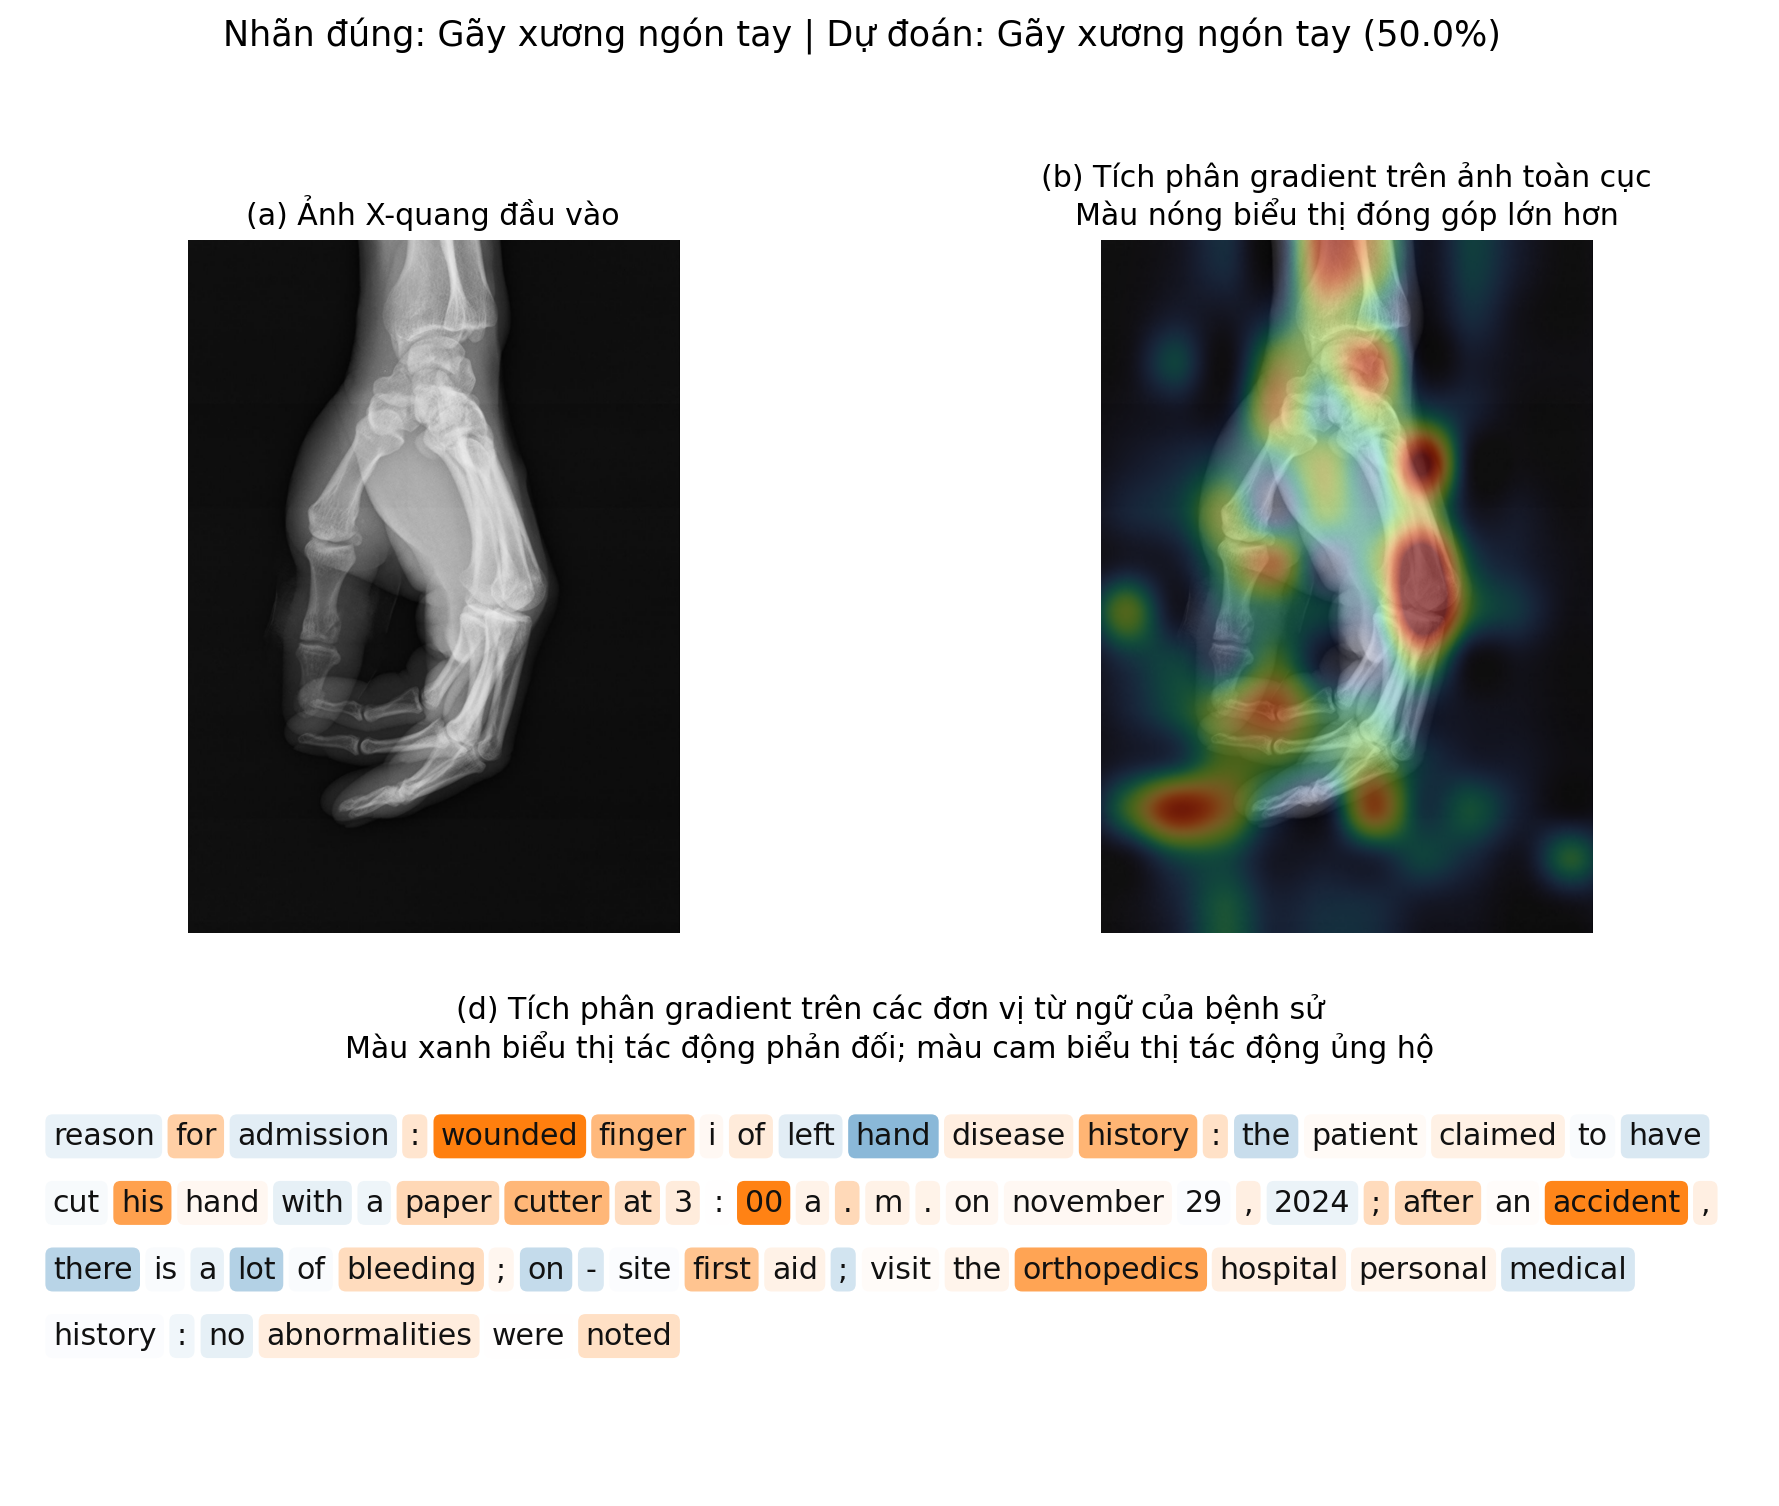
\includegraphics[trim={75.19591bp 229.18752bp 439.57607bp 95.99477bp},clip,width=\linewidth]{ig_case_source.png}
\end{minipage}\hfill
\begin{minipage}[t]{0.185\linewidth}
\centering\vspace{0pt}
{\footnotesize\textbf{(b) Image IG}}\par\smallskip
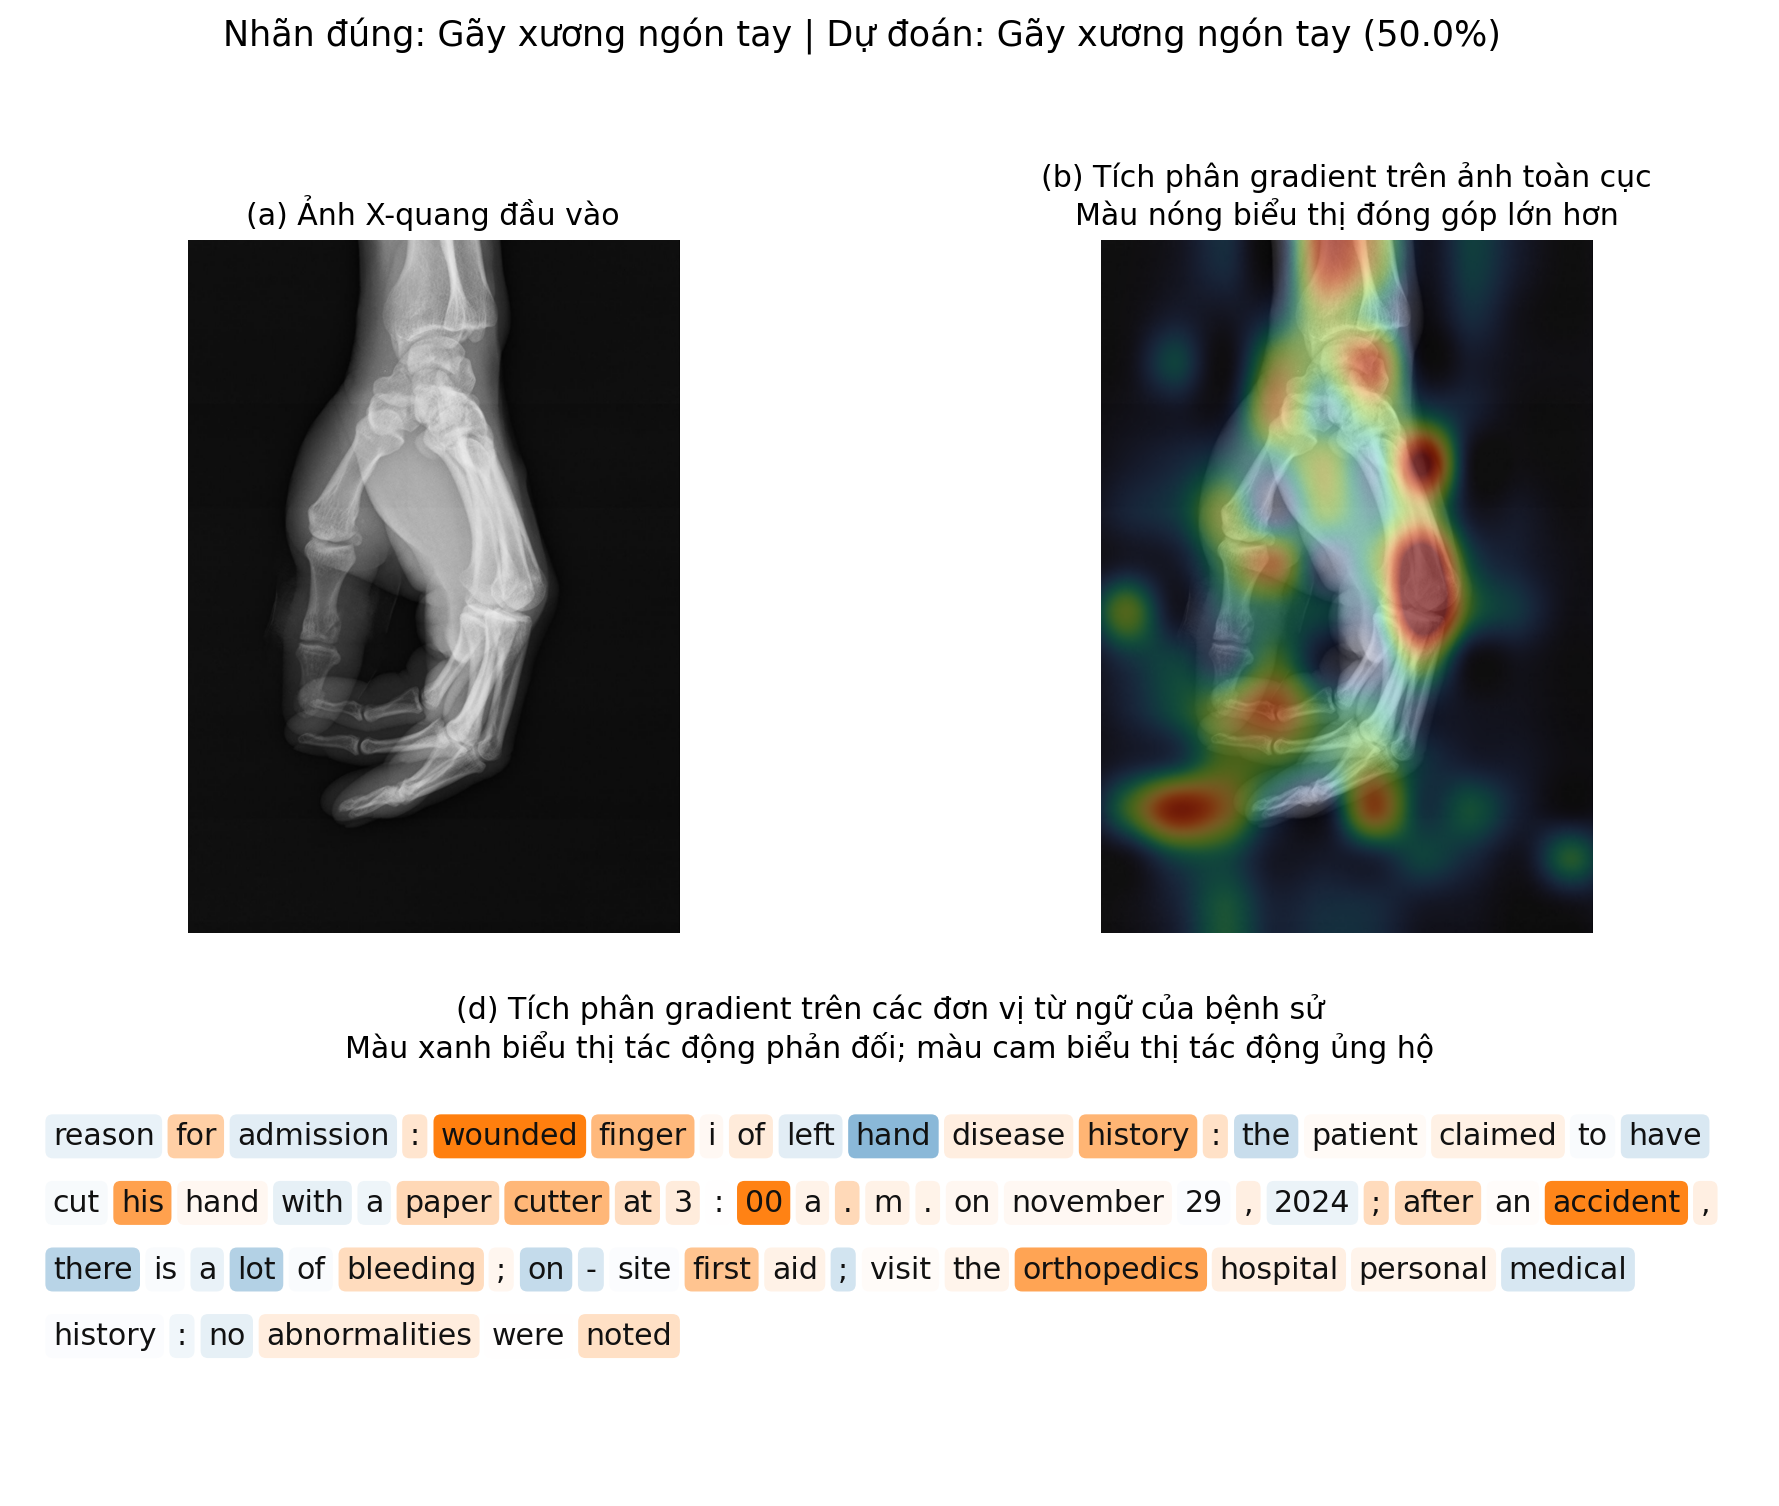
\includegraphics[trim={440.37602bp 229.18752bp 74.39595bp 95.99477bp},clip,width=\linewidth]{ig_case_source.png}
\end{minipage}\hfill
\begin{minipage}[t]{0.59\linewidth}
\raggedright\vspace{0pt}
{\footnotesize\textbf{(c) Clinical-text IG}}\par\smallskip
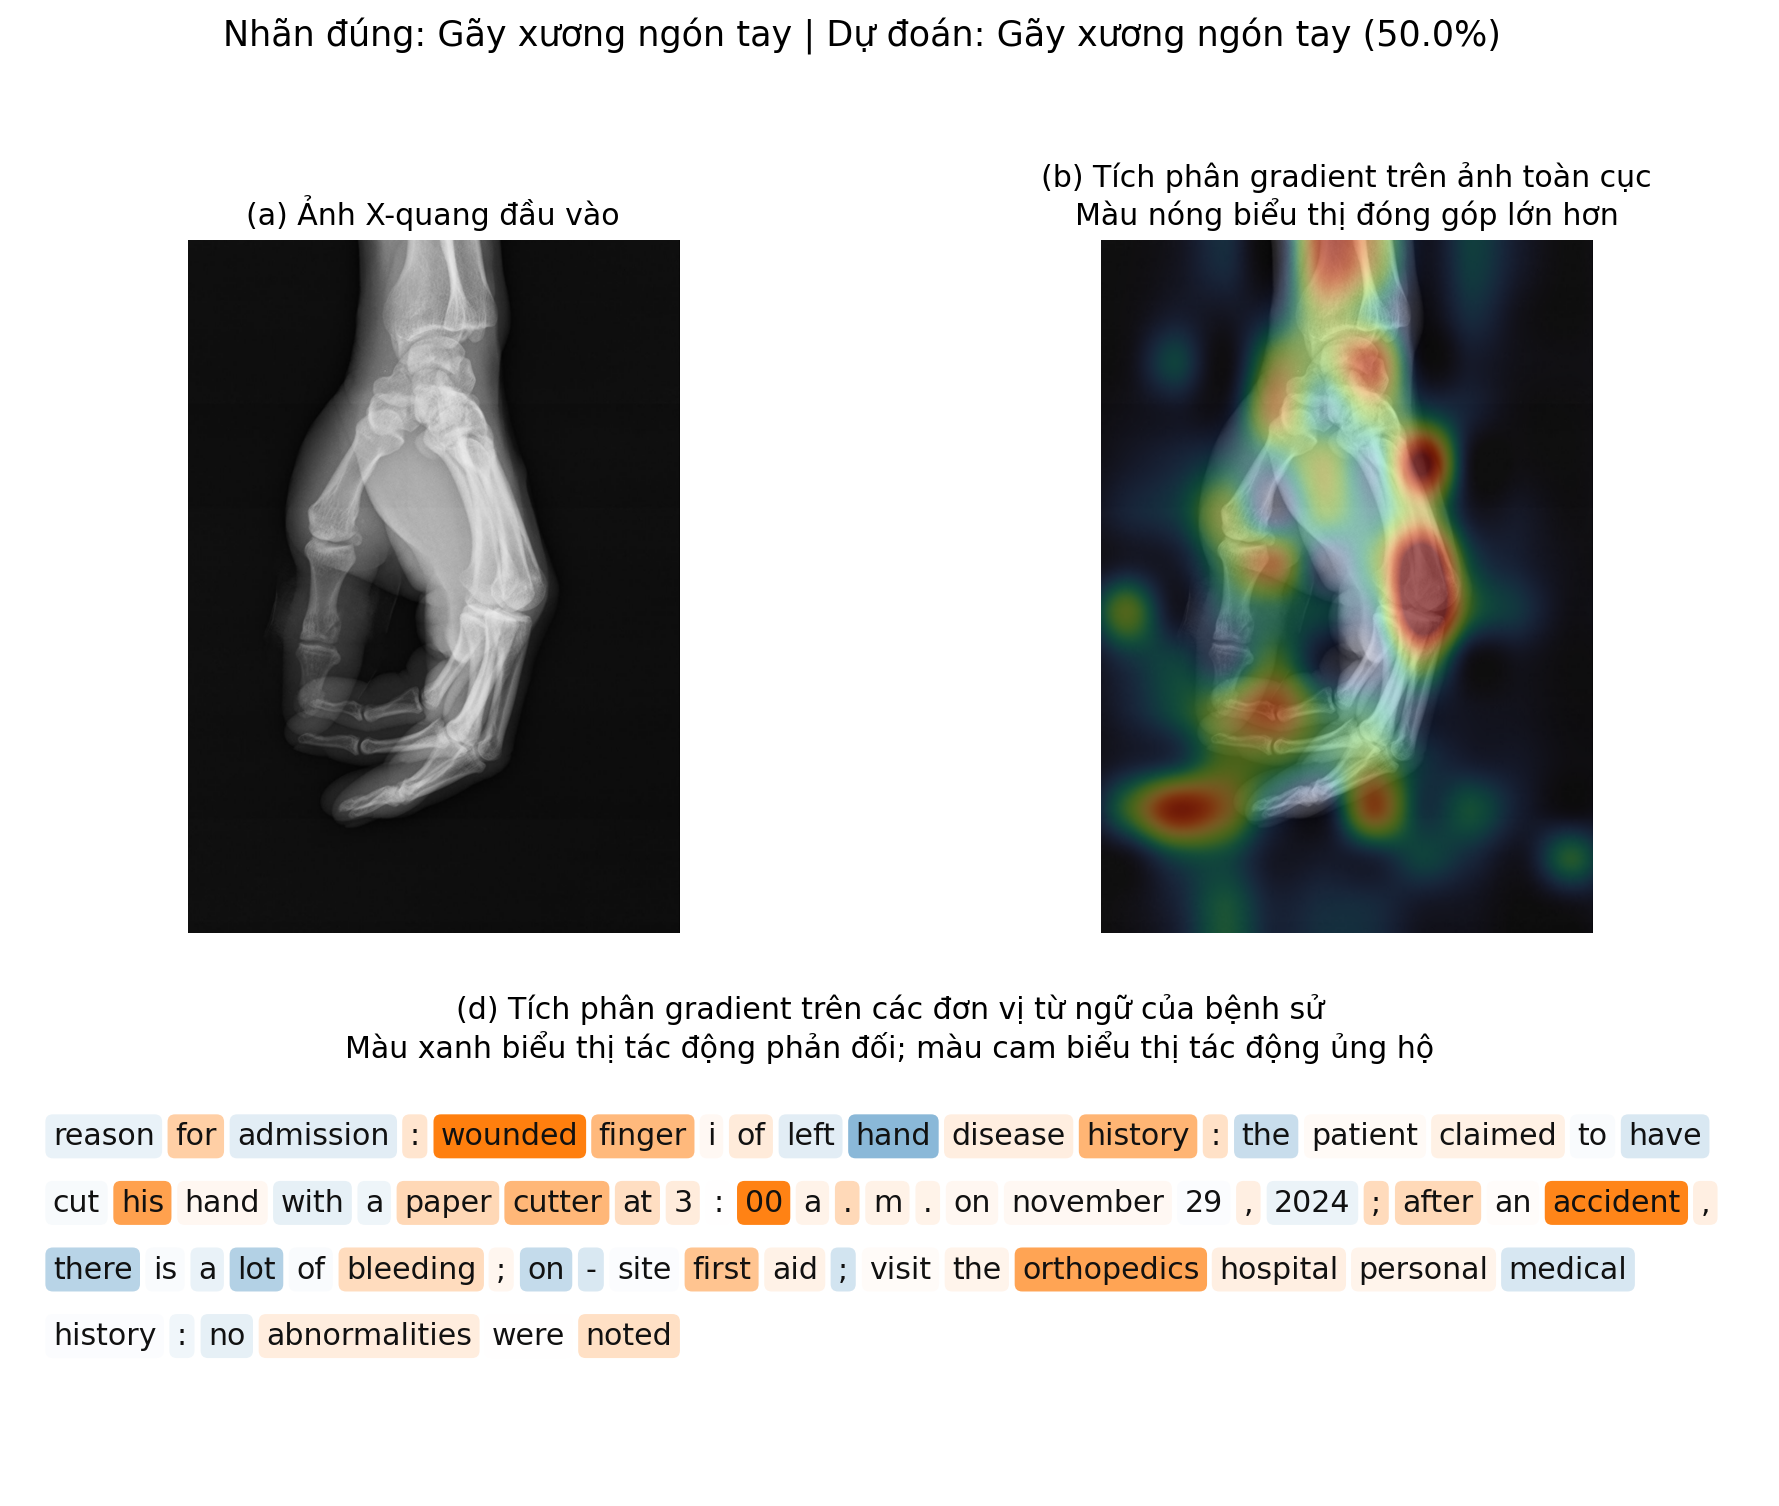
\includegraphics[trim={17.19906bp 137.99249bp 373.57966bp 444.77578bp},clip,width=0.926097\linewidth]{ig_case_source.png}\\[-1pt]
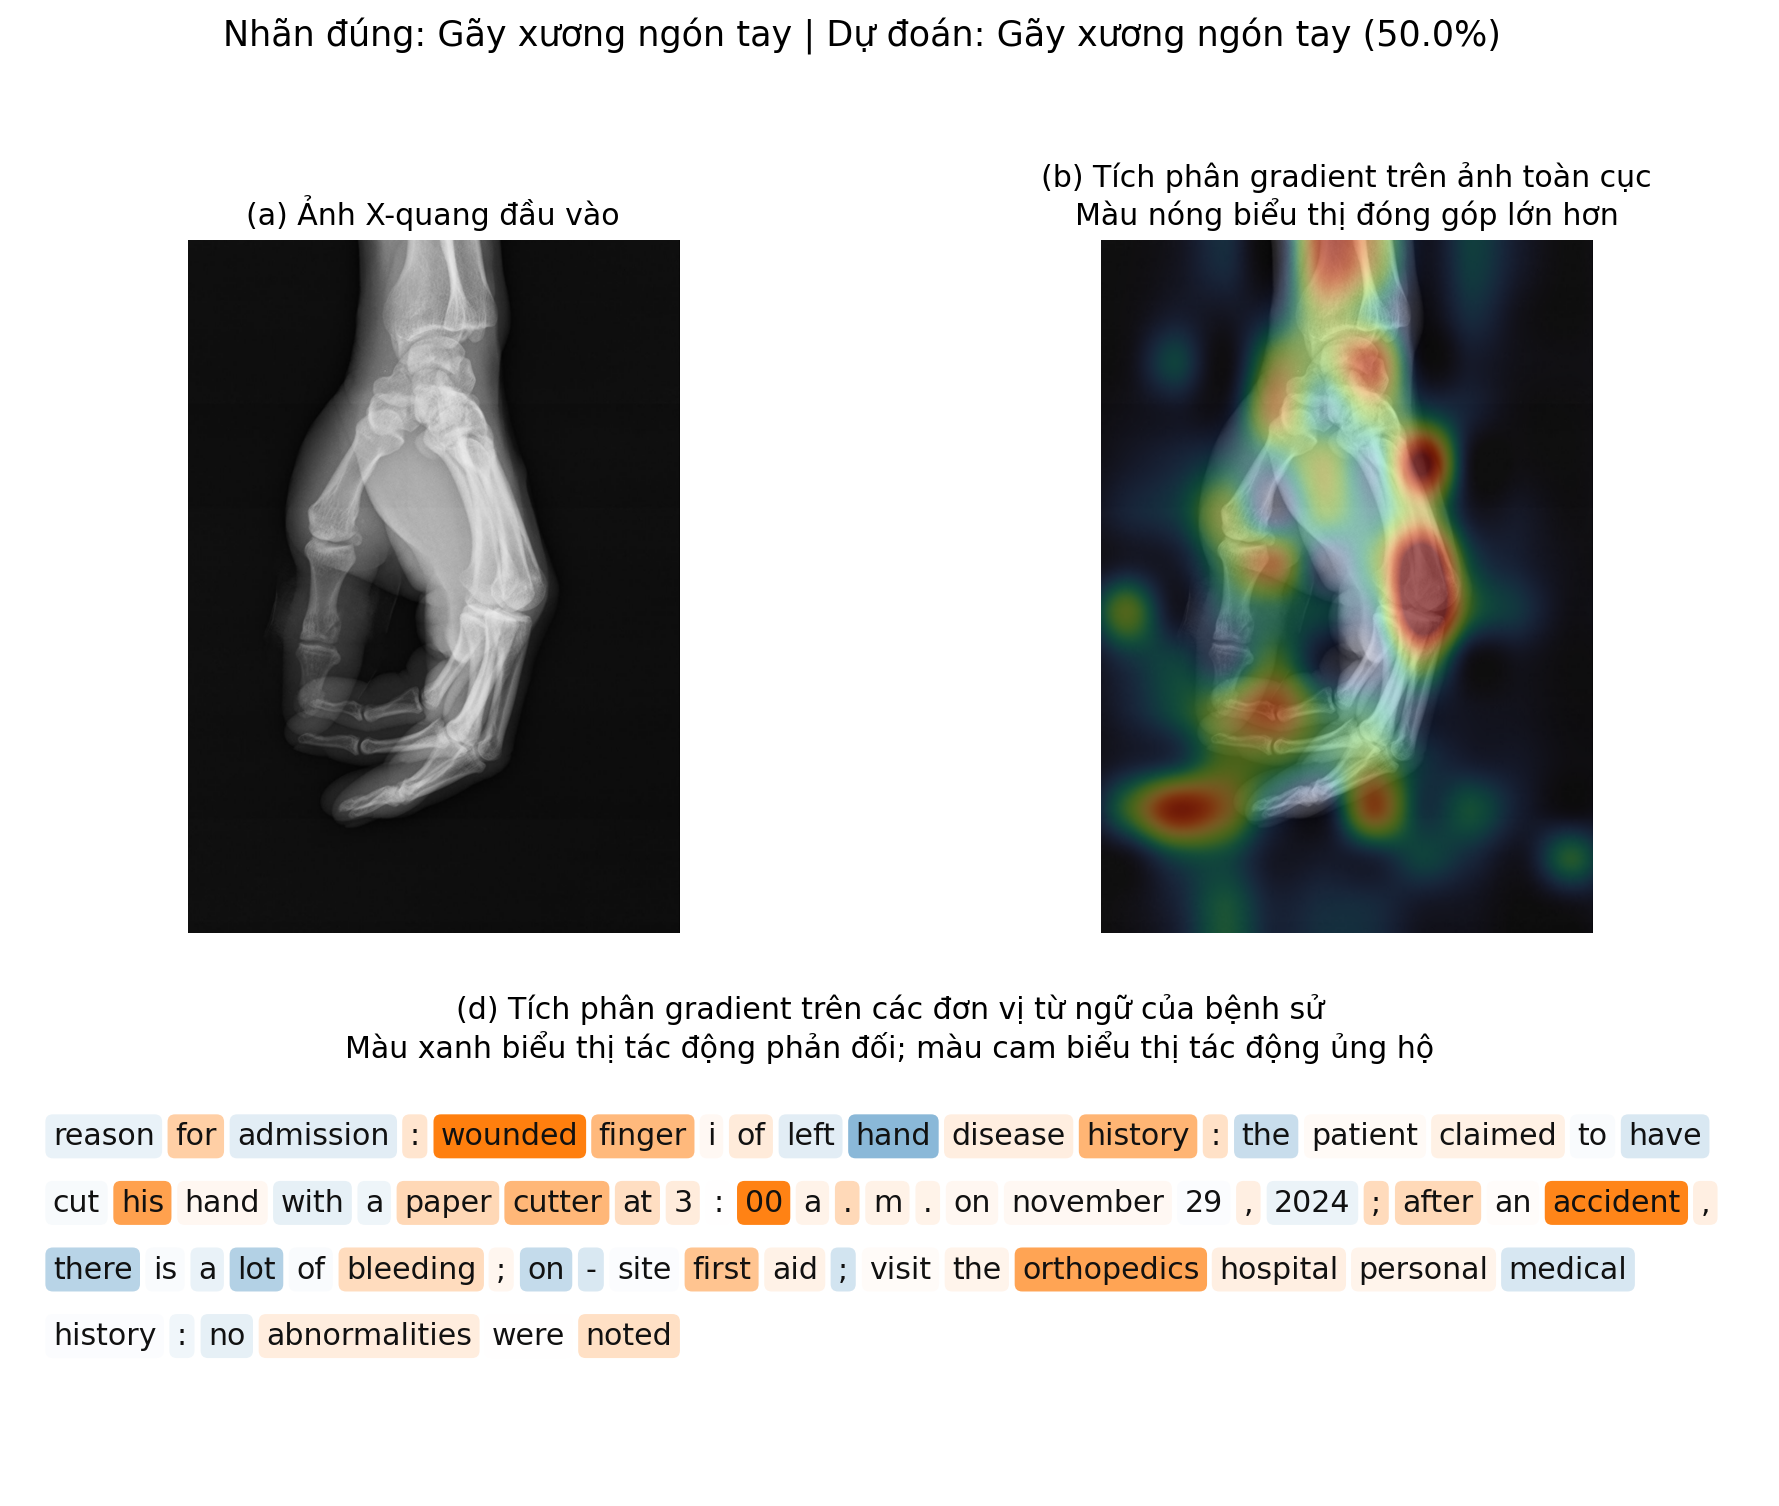
\includegraphics[trim={338.38158bp 137.99249bp 26.79854bp 444.77578bp},clip,width=1.000000\linewidth]{ig_case_source.png}\\[-1pt]
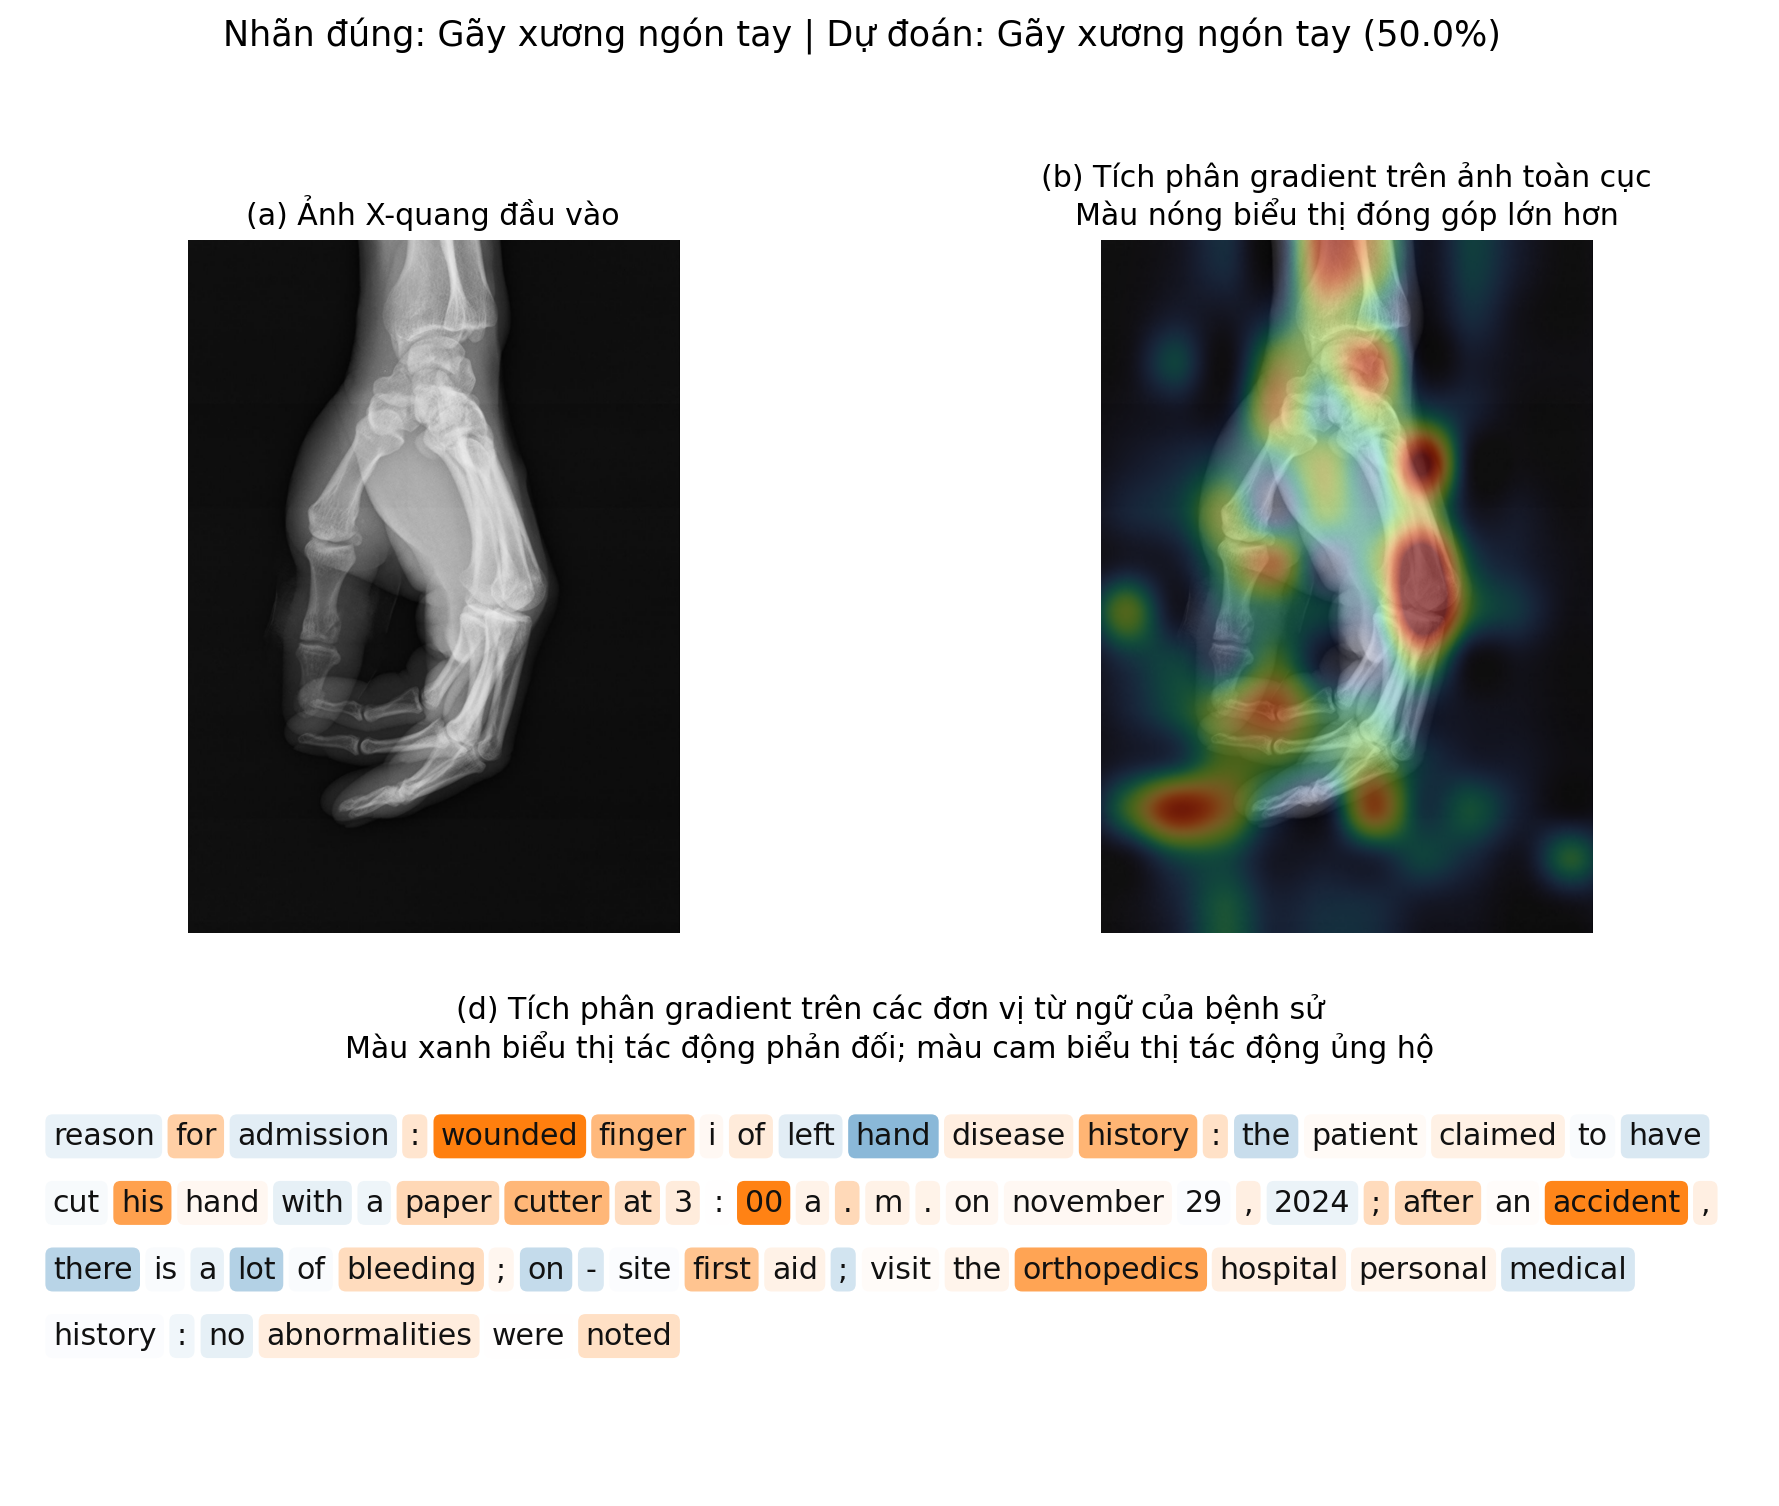
\includegraphics[trim={17.59904bp 111.59392bp 366.78003bp 471.17435bp},clip,width=0.944573\linewidth]{ig_case_source.png}\\[-1pt]
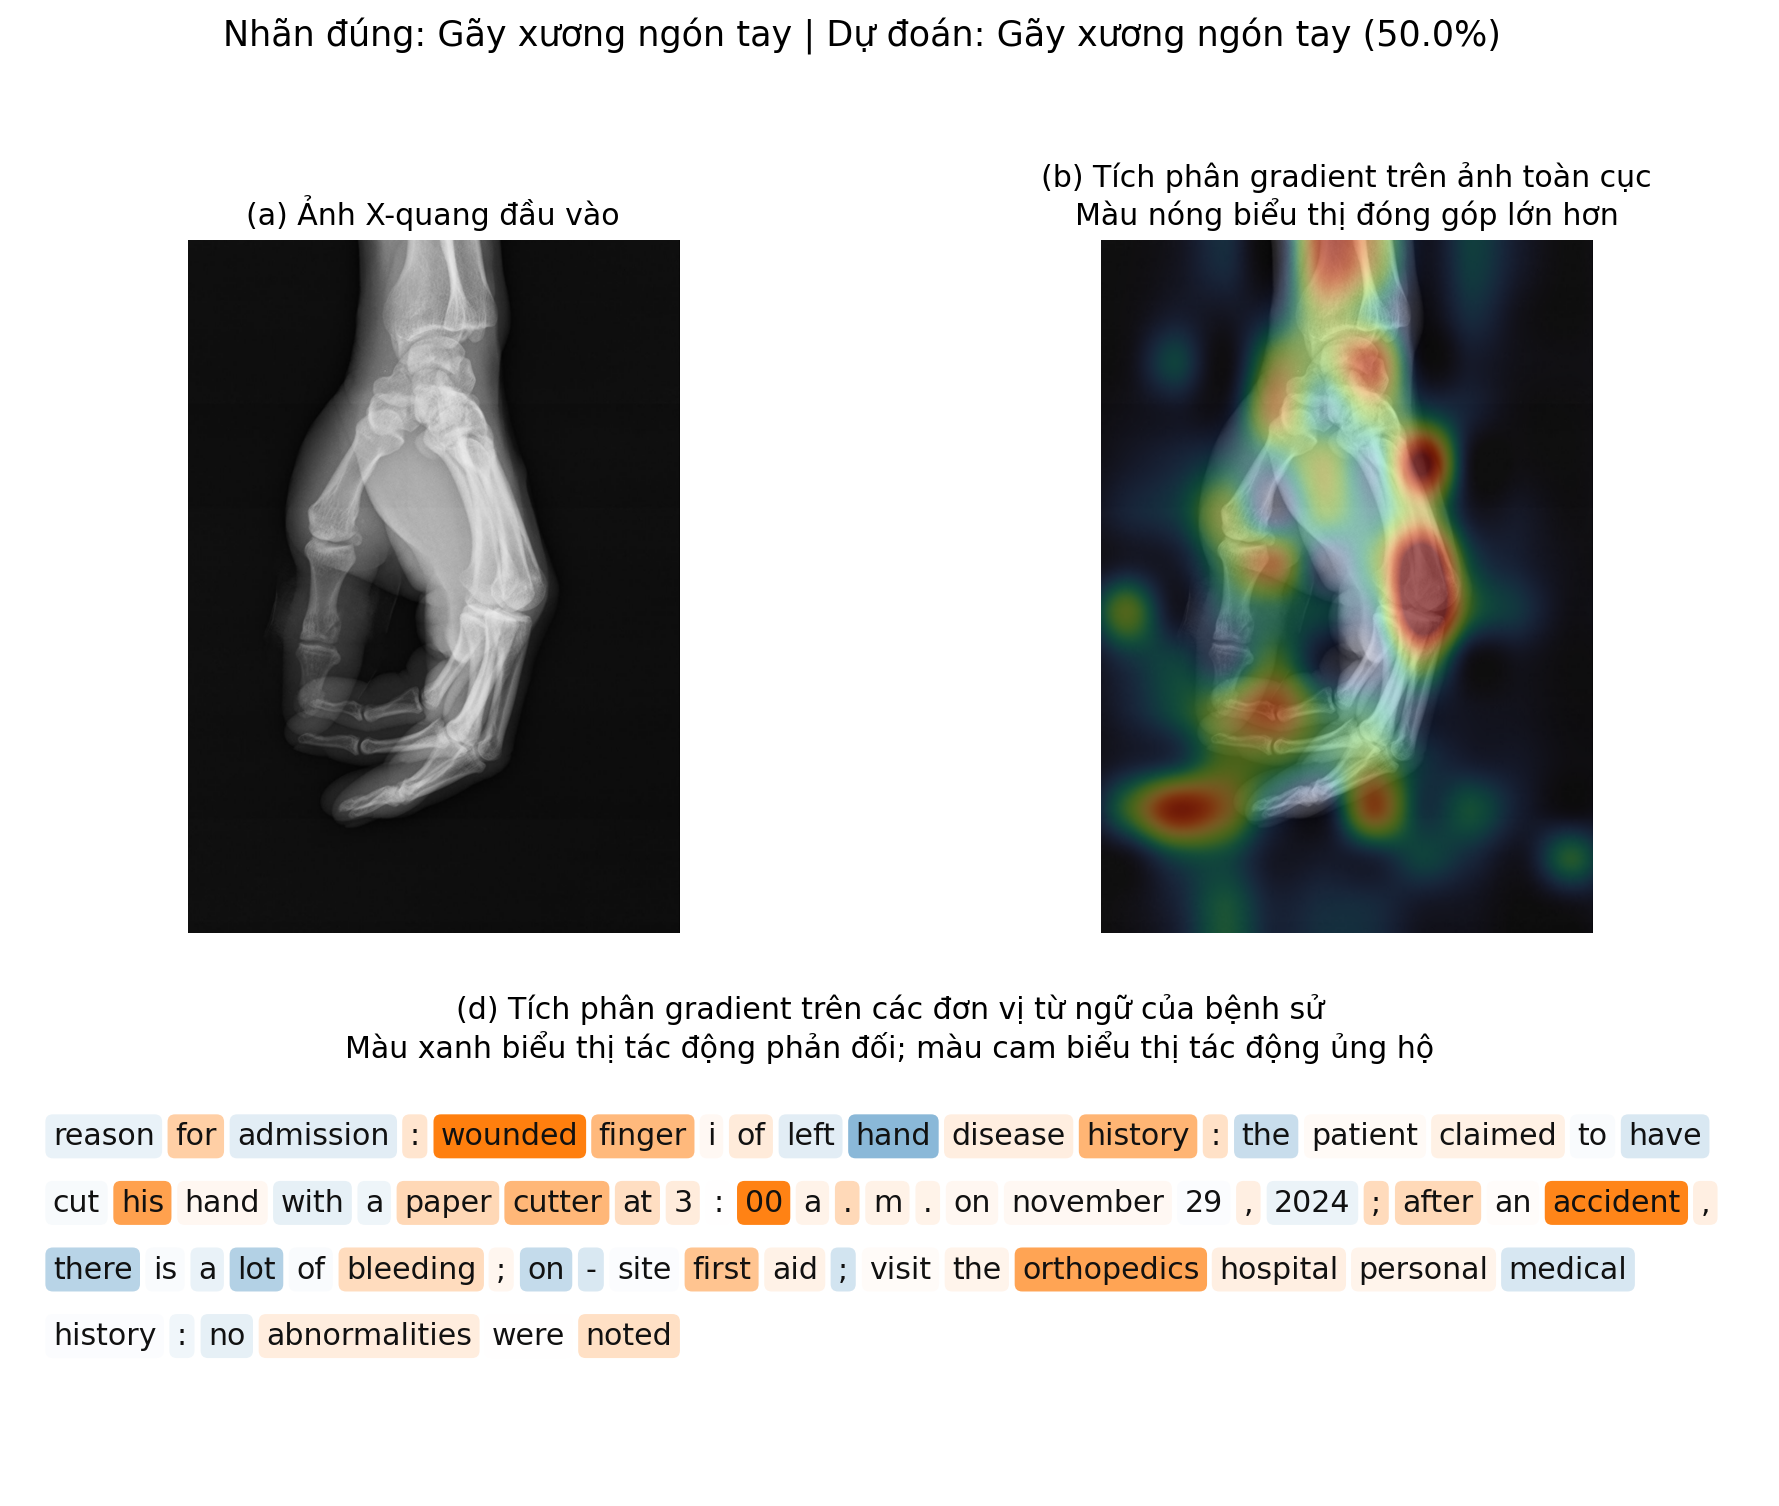
\includegraphics[trim={345.18121bp 111.59392bp 23.59872bp 471.17435bp},clip,width=0.989607\linewidth]{ig_case_source.png}\\[-1pt]
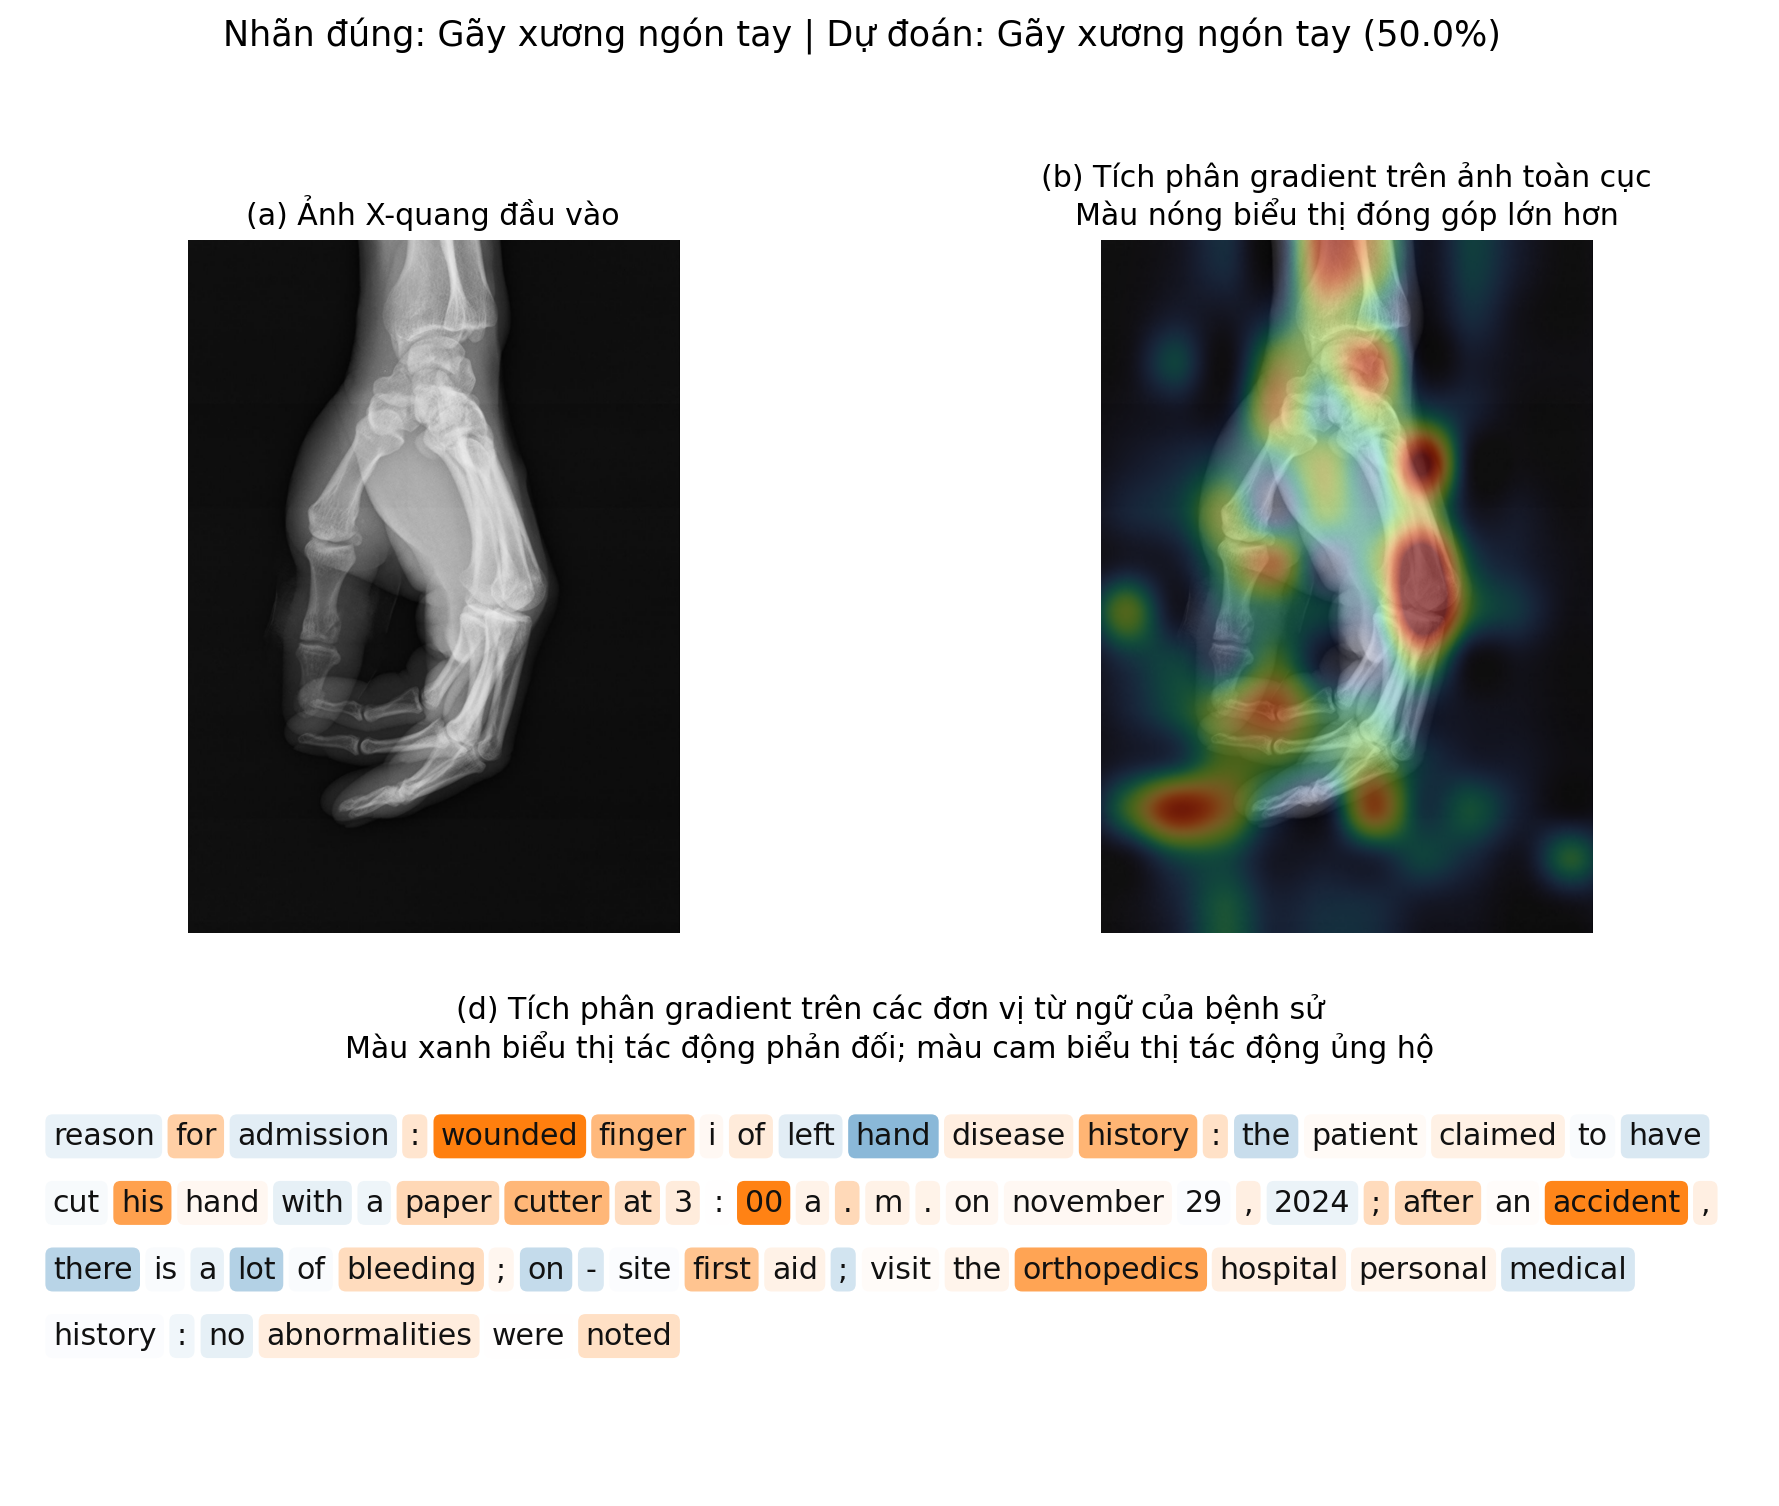
\includegraphics[trim={17.19906bp 84.79538bp 368.37994bp 497.97289bp},clip,width=0.941109\linewidth]{ig_case_source.png}\\[-1pt]
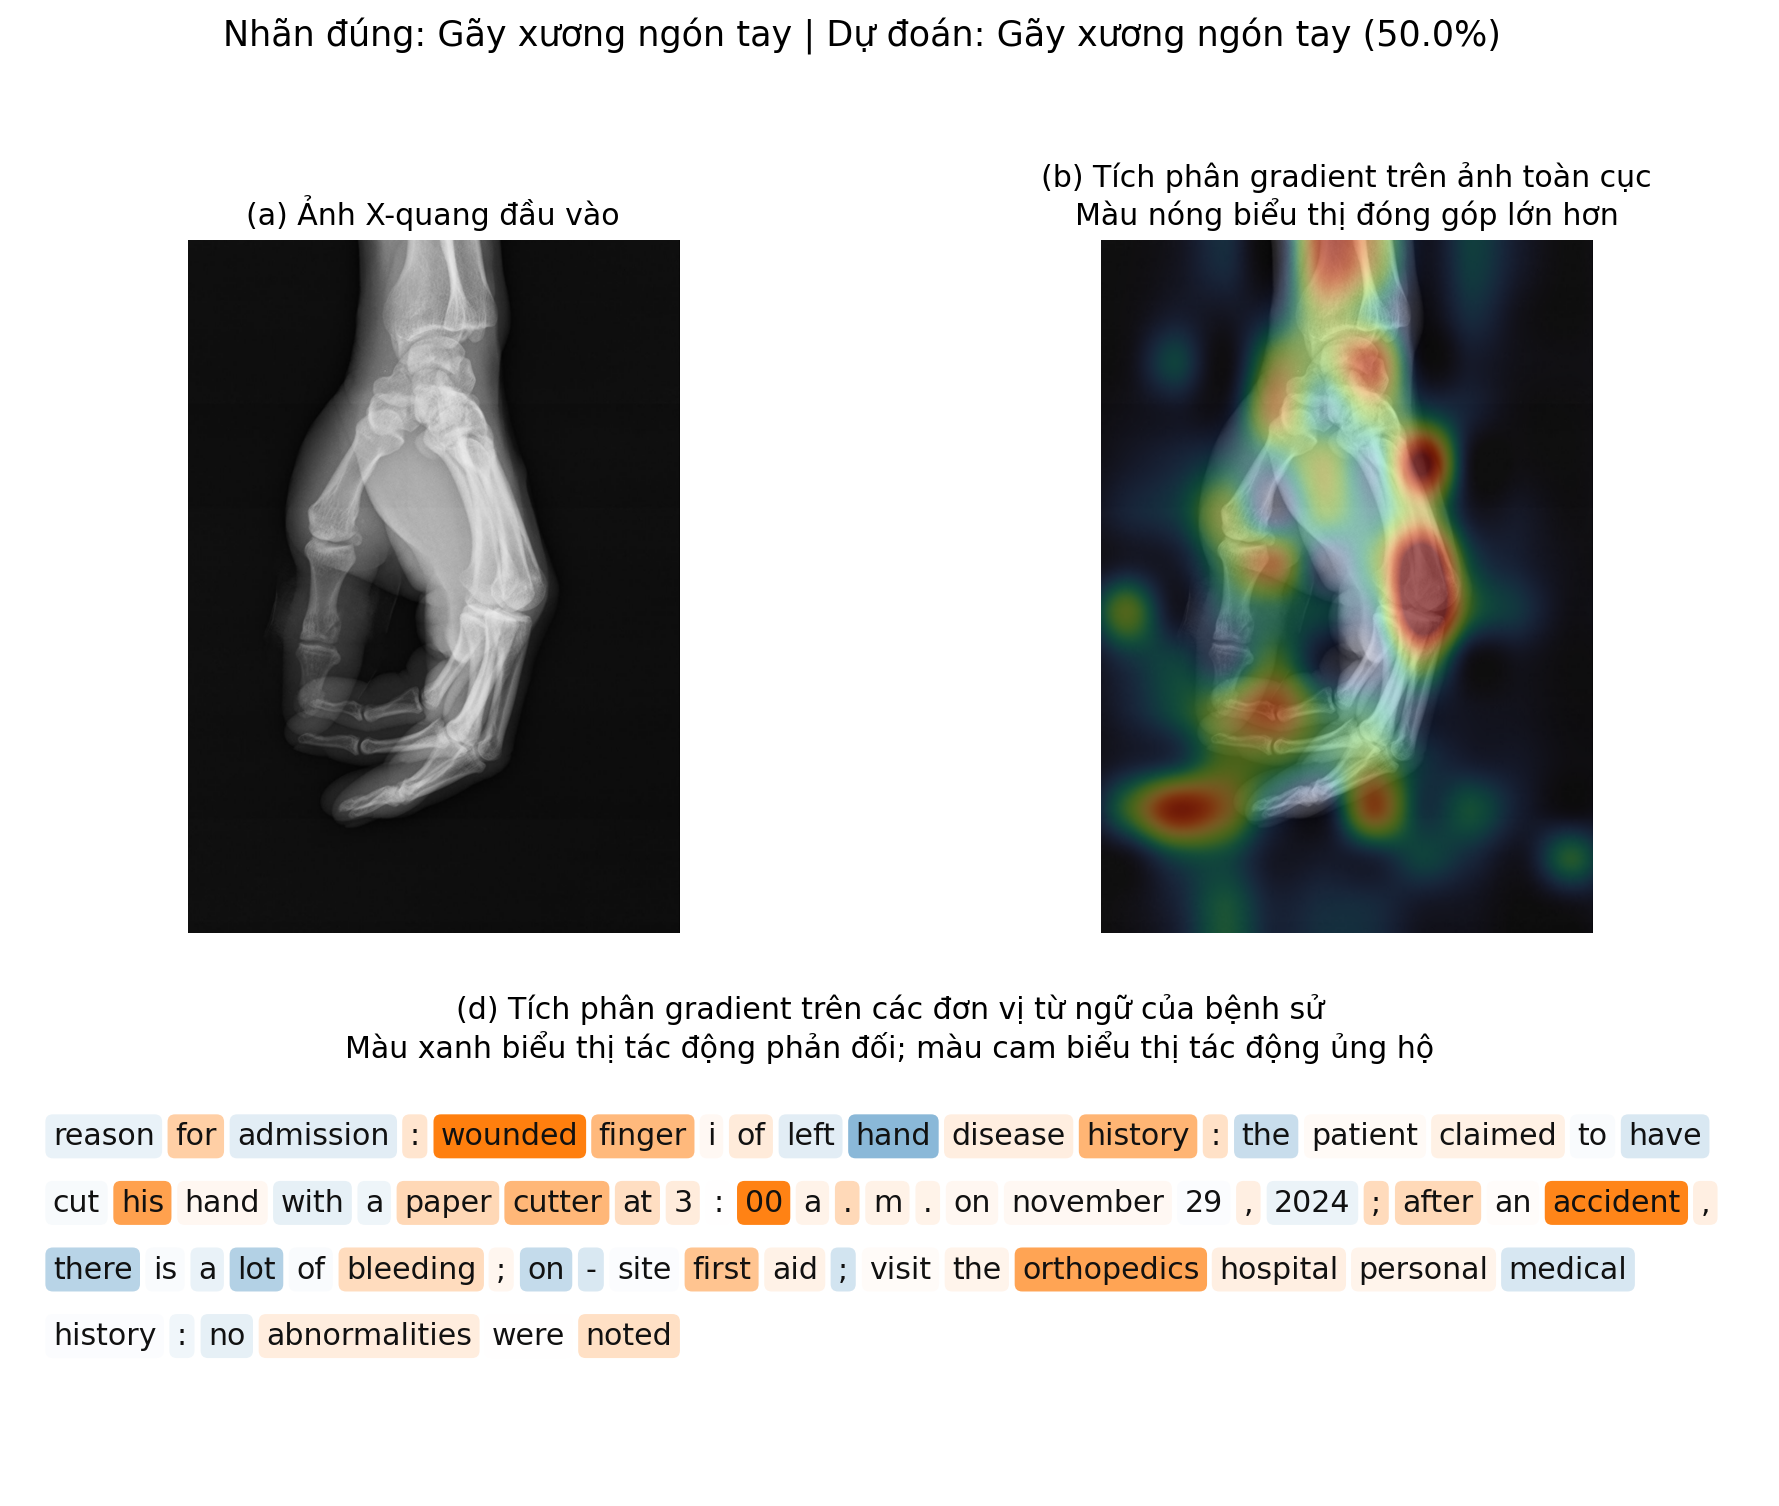
\includegraphics[trim={347.18110bp 84.79538bp 56.79691bp 497.97289bp},clip,width=0.887991\linewidth]{ig_case_source.png}\\[-1pt]
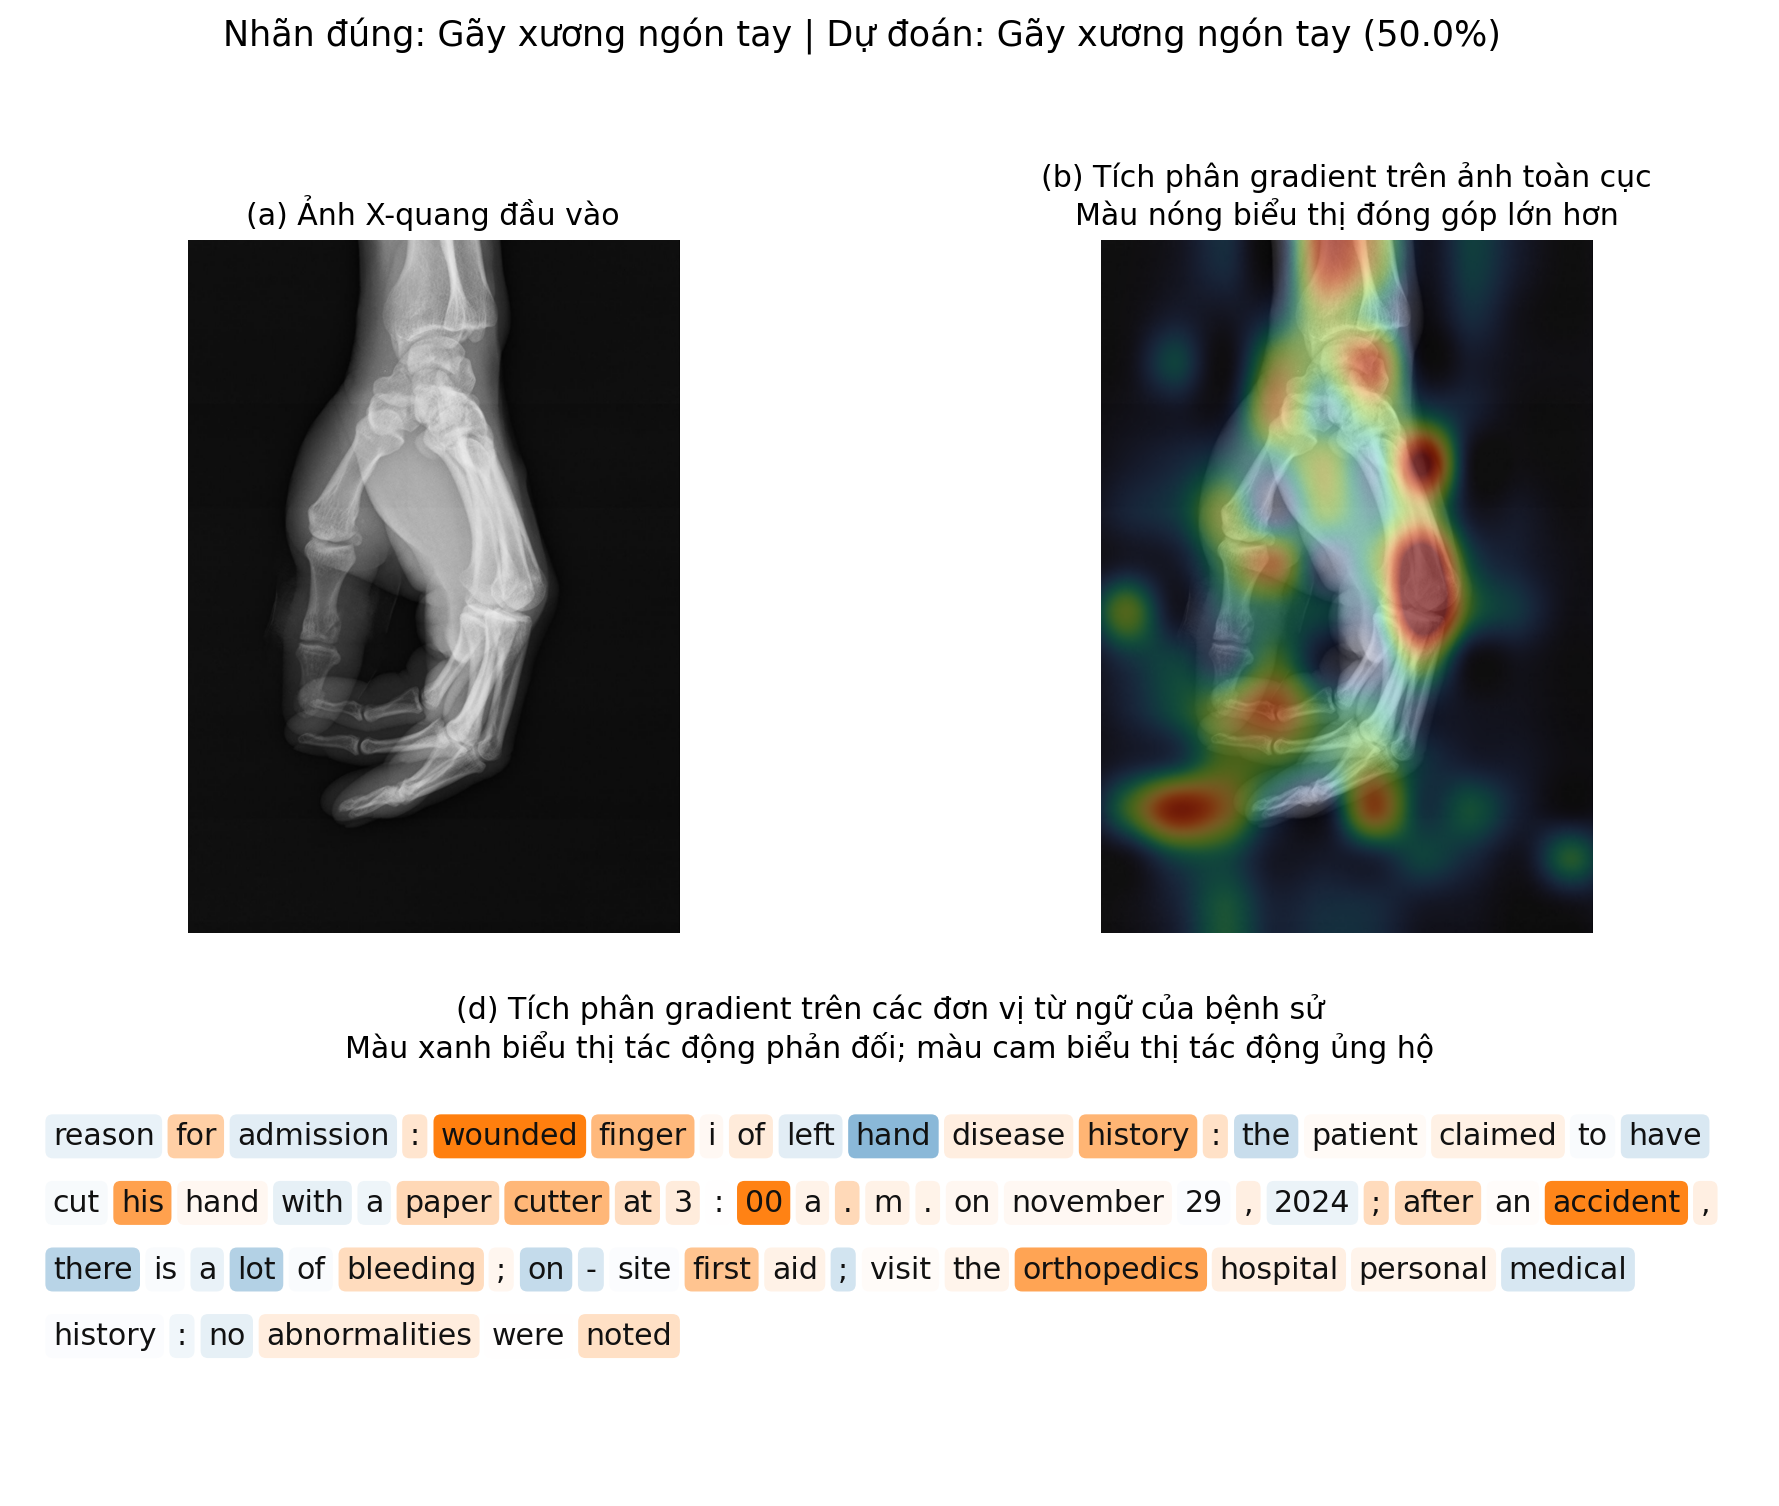
\includegraphics[trim={21.59882bp 58.39682bp 438.77611bp 524.77143bp},clip,width=0.725173\linewidth]{ig_case_source.png}\\[-1pt]
{\scriptsize\textcolor{blue!65!black}{Blue: opposing}\quad
\textcolor{orange!85!black}{Orange: supporting}}
\end{minipage}
\par\endgroup

\caption{Qualitative IG for CTCH case 3563 (XBone-Net, seed 42). Warm image colors indicate greater displayed relevance. Orange and blue text respectively support and oppose the predicted-class logit. Each attribution holds the other modality fixed. This selected example does not establish lesion localization.}
\label{fig:ig_case}
\end{figure*}

